Die Nutzung von EC2-Instanzen ist mit einem Zahlungsmodell verbunden. Die Wahl des Zahlungsmodells ist von entscheidender Bedeutung, um den besten Preis für EC2-Instanzen zu erzielen.
%EC2 and RDS(DB) spend are often on of the main portions of your overall AWS Bill t.ly/Mqwn
Die von Amazon Web Services angebotenen Zahlungsmodelle werden im Folgenden dargestellt.
\\\\
Das \textit{On-Demand-Modell} beinhaltet keine langfristigen Verpflichtungen, es ist daher die teuerste Alternative, die auf Stundenbasis berechnet wird. Die Modelle \textit{Saving Plans} und \textit{reservierte Instanzen(Reserved Instances)} erfordern den Abschluss von Verträgen über ein oder drei Jahre, um günstige Preise zu erhalten. \textit{EC2-Spot-Instanzen} sind das kostengünstigste Modell, sie haben aber den Nachteil, dass ihre Verfügbarkeit nicht immer garantiert ist. Somit weist jedes Zahlungsmodell seine Vor- und Nachteile auf und eignet sich für unterschiedliche Anwendungsfälle.\footnote{In dieser Arbeit wird nicht darauf eingegangen, wie die richtige Server-Instanz ausgewählt werden sollte, da die Auswahl von individuellen Anforderungen abhängt, die von Fall zu Fall unterschiedlich sind. Im Allgemeinen wird empfohlen, Instanzen so nahe wie möglich an den AWS-Diensten, mit denen sie kommunizieren werden, zu platzieren.} Gute Ergebnisse können auch durch die Kombination mehrerer Zahlungsmodelle erzielt werden.\footnote{Dieser Aspekt wird in Unterkapitel \ref{sssec:AWS-EC2-Fleet} ausführlicher dargestellt.} %SAG DER CLOUD-EXPERT/FIRMA 
%[WIRD ES?]
\\\\
%[IST DIESE ERKLÄRUNG NÖTIG?]
% Ressourcen vs Cloud-Dienste sollte gekläert werden
Die beste Leistung wird außerdem angestrebt, indem sich diese Instanzen in räumlicher Nähe zur Mehrzahl der Endnutzer, befinden. 
%Vor- und Nachteile noch tabellarisch aufzulisten??
%https://youtu.be/Q5wSvUVPyYY?t=678
%Excess capacity/Spot Instances
\subsection{On-Demand-Instanzen}
Bei diesem Zahlungsmodell besteht keine Notwendigkeit, ein festes Anfangsbudget festzulegen. Die Kosten richten sich nach dem Verbrauch auf der Grundlage der Nutzungsstunden. Dieses Modell eignet sich für Projekte, deren Entwicklung unvorhersehbar ist und die Möglichkeit besteht, dass das es in kurzer Zeit abgeschlossen sein wird, sodass es nicht Sinnvoll ist, eine langfristige Verpflichtung einzugehen.\footnote{Vgl. AWS, 2019, Amazon Elastic Compute Cloud - Benutzerhandbuch für Linux-Instances, S.344\cite{AMZ26}.}
\\\\
Die Preise beim dem On-Demand Zahlungsmodell variiert je nach Instanz Typ, Region und der übertragenen Datenmenge.\footnote{Die aktuellen Preise für die verschiedenen Regionen sind auf der AWS-Website in der Sektion EC2 - On-Demand-Preise zu finden. Vgl. AWS On-Demand Instances Pricing.\cite{AMZ02}} In der \autoref{fig:OnDemand_Preise} werden Preisbeispiele für die Region Ohio verfügbaren Linux-Instanzen gezeigt.\\
\begin{figure}[h!]
    \centering
    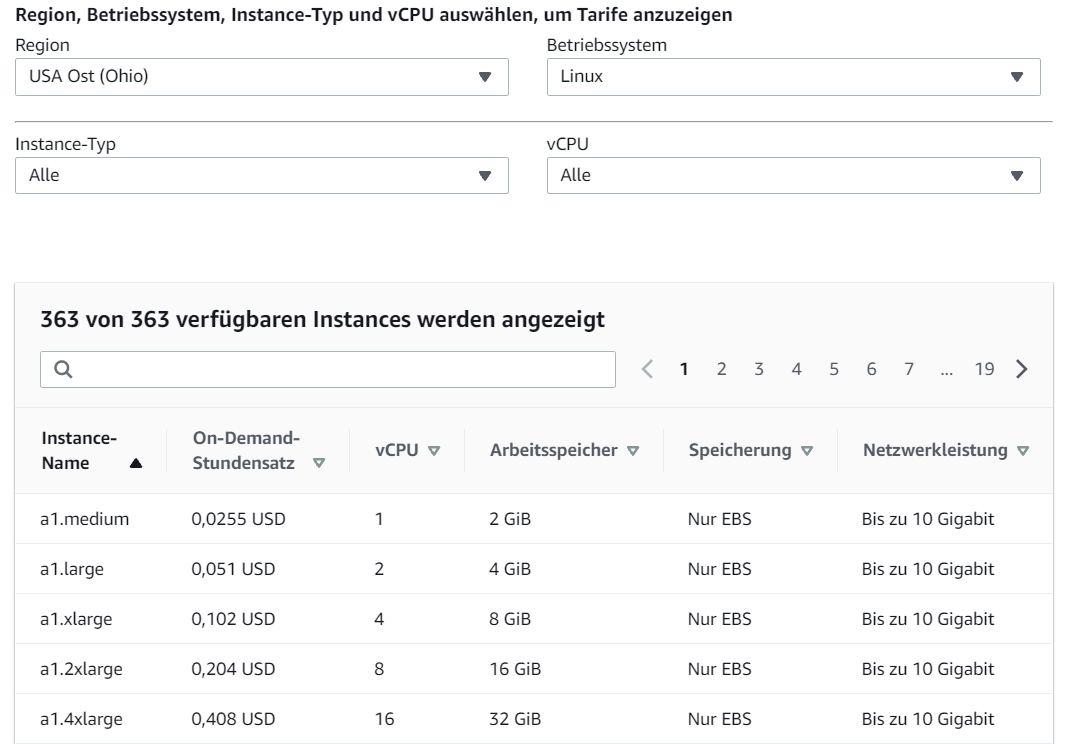
\includegraphics[scale=0.5]{sources/On-Demand-Pläne für Amazon EC2}\label{fig:OnDemand_Preise}\\
    \caption[On-Demand Preise für Amazon EC2]{}
    \label{fig:OnDemand_Preise}  
    On-Demand Preisbeispiele von EC2-Instanzen.\\
    Quelle: AWS Pricing Calculator for EC2, 2021, o.S, \cite{AMZ02}.
  \end{figure}
\\
%Aus der Abbildung geht eindeutig hervor, dass ....... Preise aufweisen. 
Es ist zu beachten, dass Instanzen mit denselben Eigenschaften (Instanz-Familie, Arbeitsspeicher, Netzwerkleistung usw.), aber in verschiedenen Regionen, unterschiedliche Preise haben können.
%WARUM IST DIESE ABB.?
\subsection{Reservierte Instanzen und Saving Plans}
%t.ly/JUWq
%https://www.youtube.com/watch?v=c_zlPQimrvY
Die Zahlungsmodelle \textit{Reservierte Instanzen} und \textit{Saving Plans} sind sich sehr ähnlich. Beide kommen mit einer gleichbleibenden  Nutzungsverpflichtung, die in US-Dollar pro Stunde gemessen wird.\footnote{AWS-Dienste werden in US-Dollar abgerechnet. Zahlungen in anderen Währungen sind auch möglich. Quelle: AWS, AWS-Console in Kontoeinstellungen, 2021, o.S.} Um die reduzierten Preise  zu bekommen, müssen Verträge über ein oder drei Jahre abgeschlossen werden. 
\\\\
\autoref{fig:EinsparungenRISP} zeigt die möglichen Einsparungen je nach Zahlungsmodell. Die Einsparungen hängen davon ab, ob man die Instanz-Familie und die Verfügbarkeitszone später verändern kann oder nicht. Je geringer die Flexibilität für spätere Änderungen, desto höher die Einsparungen.
\begin{figure}[h!]
  \centering
  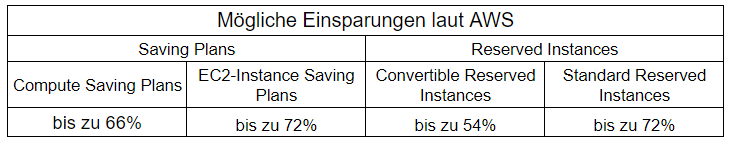
\includegraphics[scale=0.8]{sources/EinsparungenRISP}\label{fig:EinsparungenRISP}\\
  \caption[Mögliche Einsparungen bei reservierten Instanzen and Saving Plans laut AWS]{}
  \label{fig:EinsparungenRISP}
  Mögliche Einsparungen bei reservierten Instanzen and Saving Plans.\\
  Quelle: AWS, 2021, o.S., \cite{AMZ07,AMZ11}.
\end{figure}
\\
Die \textit{Compute Saving Plans} bieten die Flexibilität \textit{die Familie, die Größe, die Verfügbarkeitszone (AZ), das Betriebssystem} oder \textit{der Mandant} von EC2-Instanzen zu wechseln.\footnote{Vgl. AWS, 2021, AWS Saving Plans Pricing, o.S.\cite{AMZ11}.}\footnote{Vgl. Mark Wilkins, 2021, AWS Certified Solutions Architect - Associate (SAA-C02), S.95.\cite{AWS1}.} Diese Option ist bei \textit{EC2-Instance Saving} nicht möglich und daher bietet die zweite Option eine etwas höhere Einsparung.
\begin{quote}
    „Bei Compute Saving Plans können Sie beispielsweise jederzeit von C4- auf M5-Instances wechseln, eine Workload von EU (Irland) nach EU (London) verlagern oder eine Workload von EC2 auf Fargate oder Lambda verschieben. Dabei zahlen Sie automatisch weiterhin den Saving Plans-Preis.”
    \footnote{Vgl. AWS, 2021, AWS Saving Plans Pricing, o.S.\cite{AMZ11}.}
\end{quote}
Bei den EC2-Instance Saving Plans hingegen muss eine Instanz-Familie in einer bestimmten Region ausgewählt werden.  Dies reduziert automatisch die Kosten für die ausgewählte Instanz-Familie in der jeweiligen Region, unabhängig von Availability Zone, Größe, Betriebssystem oder Mandant.
%\\Die Festlegung eines festen Stundensatzes über einen langen Zeitraum bietet die Möglichkeit, künftige Kosten zu planen[ZITAT/WIE IM BWL ERKLÄRT]WIEDER EINBLENDEN; WENN ES SINNVOLL IST.
%-
%Folgenden Kriterien definieren den Preis von EC2-Instanzen bei SavingPlans:
%Vertraglaufzeit, Vorabzahlung, Betriebssystem,Region, Mandant
%AUCH FÜR RIs?
%3 Arten von S. Plans: Compute and EC2 Instance

%RI Configurations-Normalization https://medium.com/driven-by-code/how-truecar-saves-40-on-aws-with-ec2-reserved-instances-d0a6e0d9c08a
\subsubsection*{EC2 Reserved Instance Marketplace}\label{sssec:RI-Marketplace}
Sollte sich herausstellen, dass die Kapazität der reservierten Instanzen viel zu wenig oder gar nicht genutzt wird, kann diese Rechenkapazität auf dem \textit{RI Marketplace} (Marktplatz für den Kauf von reservierten Instanzen) zur Verfügung gestellt werden. Somit kann ein Teil der Investition zurückgeholt werden. Dies ist für Standard reservierten Instanzen möglich. Diese werden in Spot-Instanzen umgewandelt, damit andere Nutzer sie beantragen können. Dafür sollte der Instanz-Anbieter eine Servicegebühr in Betracht ziehen.\footnote{Stand November 2021 beträgt diese Gebühr 12\% (Vgl. AWS, 2021, Amazon EC2 Reserved Instance Marketplace, o.S.\cite{AMZ23}).}

\subsubsection*{Optionale Vorauszahlung}\label{sssec:Vorauszahlung}
Zusätzlich ist es bei Saving Plans und reservierten Instanzen möglich im Voraus zu zahlen. Im Gegenzug wird ein niedrigerer Gesamtpreis angeboten. AWS bietet diesbezüglich drei verschiedene Optionen an: eine teilweise, keine oder eine vollständige Vorauszahlung.\footnote{Vgl. AWS, 2021, AWS Pricing Calculator o.S.\cite{AMZ17}.} Bei teilweiser Vorauszahlung ist eine Anzahlung von etwa 50\% zu leisten.
\\\\
Die \autoref{fig:EinsparungenVorauszahlung} zeigt den Vergleich zwischen den drei Vorauszahlungsoptionen für 20 Instanzen über drei Jahren im Zahlungsmodell Saving Plan. Hier wird deutlich, dass es kaum einen Unterschied zwischen einer teilweisen und keinen Vorauszahlung gibt. Eine erhebliche Einsparung ergibt sich jedoch, wenn man für den gesamten Zeitraum der gebuchten Instanzen im Voraus bezahlt.
\begin{figure}[h!]
    \centering
    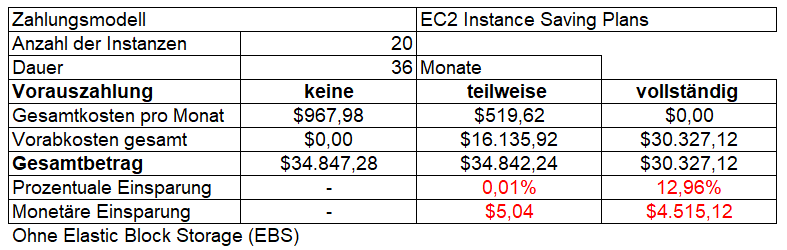
\includegraphics[scale=0.6]{sources/EinsparungenVorauszahlung}\label{fig:EinsparungenVorauszahlung}\\
    \caption[Mögliche Einsparungen durch Vorauszahlungen]{}
    \label{fig:EinsparungenVorauszahlung}
    Mögliche Einsparungen durch Vorauszahlungen für\\
    EC2 Instanzen in Saving Plans Zahlungsmodell.\\
    Eigene Darstellung. \\
    Quelle: AWS, 2021, AWS Pricing Calculator, o.S.\cite{AMZ17}.
  \end{figure}
  \\
Die Berechnungen wurden anhand des \textit{AWS Pricing Calculator} für Instanz-Familie \textit{t4g.xlarge} und in der Region EU (Frankfurt) durchgeführt.{\cite{AMZ17}} 
\\\\
\subsection{Spot-Instanzen }\label{ssec:Spot-Instances}
Wie in Unterkapitel \ref{sssec:RI-Marketplace} genannt, bieten EC2 Spot-Instanzen die Möglichkeit aus den ungenutzten EC2-Instanzen anderer Nutzer zu profitieren. Mit einem Preisvorteil von bis zu 90\% gegenüber \textit{On-Demand-Instanzen} sind \textit{Spot-Instanzen} ideal für fehlertolerante Anwendungen, wie auf \textit{Containern} ausgeführte Workloads, CI/CD, Bigdata-Anwendungen und ähnliches.

\subsubsection*{Unterbrechbarkeit}
Es ist zu beachten, dass Spot-Instanzen jederzeit unterbrochen werden können. Einer der Gründe ist die Preisüberschreitung der Instanz. Wenn Spot-Instanzen angefordert werden, wird einen Maximalpreis festgelegt. Ist der Preis der Spot-Instanz höher als der angegebene Maximalpreis, ist die Spot-Instanz für die aktuelle Einstellung nicht mehr verfügbar. Ein anderes Szenario tritt ein, wenn der Instanz Anbieter die Spot-Instanz erneut anfordert. Falls eine Spot-Instanz unterbrochen wird, benachrichtigt AWS den aktuellen Nutzer darüber zwei Minuten im Voraus. Dieses Ereignis ist ebenfalls auf \textit{CloudWatch} verfügbar, damit weitere Alarme eingestellt werden können.\footnote{Diese und andere Funktionalitäten von CloudWatch werden in Kapitel \ref{kap_kostenueberwachung} näher erläutert.} Da Spot-Instanzen anfällig für Unterbrechungen sind, ist es nicht empfehlenswert, für Produktionsumgebungen nur Spot-Instanzen zu verwenden.
%Um von der Preisvorteile der Spot-Instanzen zu profitieren und Ausfälle zu vermeiden, sollten in Kombination weitere Zahlungsmodelle verwenden werden.
%\\
%Zum Beispiel eine Kombination aus Spot-Instanzen für die erwarteten Last und On-Demand-Instanzen für die dynamischen Last.
%https://aws.amazon.com/de/ec2/spot/pricing/

%2 OPTIONEN: LOWEST PRICE OR DIVERSIFIED ACROSS n POOLS TO AVOID DOWNS https://www.linkedin.com/learning/aws-automation-and-optimization/request-spot-instances-part-2?autoAdvance=true&autoSkip=true&autoplay=true&resume=false&u=79182202

\subsection{Amazon EC2 Fleet} \label{sssec:AWS-EC2-Fleet}%[Rev]
\textit{Instanzen-Flotten} oder auf Englisch \textit{fleet of instances}, bieten bei AWS die Möglichkeit mehrere Spot-Instanzen anzufordern, um einen bestimmten Bedarf an Rechenleistung zu decken.\footnote{Vgl. AWS, 2019, Amazon Elastic Compute Cloud - Benutzerhandbuch für Linux-Instances, S.708\cite{AMZ26}.} Spot-Instanzen können aber auch für produktive Umgebungen verwendet werden.\footnote{Vgl. Isaac Vallhonrat, 2020, Running Web Applications on Amazon EC2 Spot Instances, o.S.\cite{AMZ24}.} Darüber hinaus ist es empfehlenswert, Instanzen aus verschiedenen Zahlungsmodellen zu kombinieren, um von den Einsparungen von der verwendeten Spot-Instanzen, Saving Plans und reservierten Instanzen zu profitieren. Die Kombination von Instanzen aus verschiedenen Zahlungsmodellen auf Produktionsumgebungen wirkt dem Nachteil entgegen, der mit Spot-Instanzen verbunden ist. Da, bei Unterbrechung von Spot-Instanzen, bleiben noch Instanzen anderer Zahlungsmodelle weiterhin in Betrieb.
\\\\
Folgende Punkte sind für die Nutzung von Spot Fleet Instanzen zu berücksichtigen:
\subsubsection*{Wahl der Spot-Instanzen}
Die zu berücksichtigenden Instanzen für die Instanzen-Flotte, müssen den Anforderungen der %jeweiligen 
Applikation entsprechen. Um die Wahrscheinlichkeit zu erhöhen, dass mehr Spot-Instanzen gefunden werden, ist es daher empfehlenswert, die Kriterien der Suche zu erweitern. Dies kann erreicht werden, indem Instanzen ähnlicher Typen einbezogen werden. Die Berücksichtigung von den Instanzen-Familien, welche eine höhere Leistung aufweisen als erfordert wird, ist ebenfalls eine gute Option. Da in diesem Falle der Preis für Spot-Instanzen trotz höherer Leistung geringer sein wird, als der von den On-Demand-Instanzen\cite{AMZ24}. 
%Alte Version: . Denn, obwohl die Leistung die Anforderungen der Applikation überstiegen werden, wird es einen reduzierten Preis für die Spot-Instanzen bezahlt als bei On-Demand Zahlungsmodell.

\subsubsection*{Maximaler Stundenpreis}
Wie im Unterkapitel \ref{ssec:Spot-Instances} erwähnt, muss für die Anforderung von Spot-Instanzen ein Maximalpreis festlegt werden. In diesem Fall ist die Festlegung dieses Maximalpreises auch für die gesamte Instanzen-Flotte eine Option. Es kann erwartet werden, dass die Spot-Preise im Laufe der Zeit stabil bleiben, da sie keinen starken Preisschwankungen unterliegen. Diese Informationen sind nur mit einem AWS-Konto zugänglich.\footnote{Die aktuellen Preis und der Preisverlauf von Spot-Instanzen können in auf der AWS-Konsole abgefragt werden. (Vgl. AWS, 2021, EC2 Spot Instanzen-Anfragen und Preisverlauf o.S. \cite{AMZ25}).}

\subsubsection*{Festlegung von On-Demand-Anteil}
Wenn alle oder eine große Anzahl von Spot-Instanzen nicht mehr verfügbar sind, muss die benötigte Rechenkapazität von Instanzen anderer Zahlungsmodellen, wie On-Demand abgedeckt werden. Die Standardeinstellungen liegen bei 70\% On-Demand-Instanzen und 30\% Spot-Instanzen.\footnote{Vgl. Isaac Vallhonrat, 2020, Running Web Applications on Amazon EC2 Spot Instances, o.S.\cite{AMZ24}} Im Fall von vorhandenen reservierten Instanzen oder Instanzen von Saving Plans werden On-Demand-Instanzen zum entsprechend reduzierten Preis berechnet.\footnote{Vgl. AWS, 2019, Amazon Elastic Compute Cloud - Benutzerhandbuch für Linux-Instances,, S.690\cite{AMZ26}.}

\subsubsection*{Auto Scaling Groups}%Sarah 6.12
Auch als \textit{Auto-Scaling-Gruppe}(ASG) bezeichnet und ist für die Skalierung der zu startenden Instanzen verantwortlich. Hierfür wird eine Startkonfiguration benötigt, welche definiert, unter welchen Bedingungen Instanzen gestartet oder beendet werden sollen. In der Startkonfiguration werden unter anderem der \textit{Instanztyp, Security-Groups,} und \textit{Tags} festgelegt.\footnote{Mehr zu dem Thema Auto-Scaling und seine verschiedenen Konfigurationen findet sich in Kapitel~\ref{kap_Optimierung}.} Für die Nutzung von EC2-Flotten und Auto Scaling-Gruppen fallen keine zusätzlichen Kosten an. Lediglich müssen die von der EC2-Instanzen verursachten Kosten getragen werden.\footnote{Vgl. AWS, 2019, Amazon Elastic Compute Cloud - Benutzerhandbuch für Linux-Instances, S.709\cite{AMZ26}. }
%\subsubsection*{Einschränkungen?[rev]}

\subsection{Anwendungsfall: TrueCar}\label{ssec:UseCaseTrueCar}
%[Rev]
Instanzen in Zahlungsmodellen, die zu zeitlichen Verpflichtungen führen, bergen die Gefahr, dass die benötigte Rechenkapazität mittel- bis langfristig falsch eingeschätzt wird. Einerseits kann die reservierte Rechnerkapazität zu gering eingeschätzt werden. Als Konsequenz daraus wird die Rechnerkapazität großenteils mit On-Demand-Instanzen abgedeckt. Diese konnte im Anteil der reservierten Instanzen berücksichtigt und mit reduzierten Preisen berechnet werden. Andererseits, wenn zu viel Rechnerkapazität mit reservierten Instanzen reserviert und diese zu wenig gebraucht wird. Besteht die Möglichkeit, dass es die reine Nutzung von On-Demand-Instanzen eine kostengünstigere Option darstellt.
\\\\
Im Folgenden wird näher auf die Strategie von \textit{TrueCar Inc.} eingegangen, durch dessen Anwendung beide der oben genannten Problematiken vermieden werden können.  
%verfolgt hat, um in keine der beiden oben genannten Situationen zu geraten. 
TrueCar Inc. ist eine Preis- und Informations-Website für Neu- und Gebrauchtwagenkäufer mit Sitz in Santa Monica, Kalifornien.%\footnote{Die Quelle dieser Informationen ist ein Artikel\cite{MED1}, der auf www medium.com veröffentlicht wurde. Dass der Artikel von TrueCar stammt, wird durch die Tatsache bestätigt, dass deren Website www.truecar.com/who-we-are/ zu dem hier erwähnten Artikel führt.}
%https://medium.com/driven-by-code/how-truecar-saves-40-on-aws-with-ec2-reserved-instances-d0a6e0d9c08a
Dank einer Optimierungsstrategie konnten sie ihre AWS-Kosten durch die Nutzung reservierter Instanzen um etwa 40\% senken.\footnote{Vgl. David Wang, 2019, How TrueCar Saves 40\% on AWS with EC2 Reserved Instances. O.s. \cite{MED1}.}
\\\\
Um eine solche Einsparungen zu erreichen, musste das Team zuerst verstehen, wie AWS-Dienste wie \textit{reservierte Instanzen, Cost-Explorer, Auto-Scaling-Gruppen} und \textit{Lambda Funktionen} funktionieren. Damit haben sie eines der häufigsten Hindernisse überwunden mit denen Unternehmen bei der Nutzung von Cloud-Diensten konfrontiert werden; den Mangel an technischem Wissen in Bezug auf Cloud-Dienste.\footnote{Vgl. Accenture Dienstleistungen GmbH. Hohe Erwartungen an die Cloud: Hürden meistern, Mehrwert maximieren, S.11\cite{ACC1}.} Nachdem das TrueCar-Team die notwendigen Informationen, insbesondere über die reservierten Instanzen, verstanden haben, wurde anschließend die benötigte Rechenkapazität ermittelt.\footnote{In dem Artikel über TrueCar wurde nicht explizit erläutert, wie die benötigte Rechnerkapazität berechnet wurde. Diese Informationen werden jedoch von Cost-Explorer angezeigt. Cost-Explorer bietet die Möglichkeit, die Nutzung der AWS-Diensten für die letzten 12 Monate anzuzeigen. Ausführlicher wird diese Thematik in Unterkapitel~\ref{ssec:Cost-Explorer} behandelt werden.} Die Kosten der Instanzen in On-Demand wurden mit dem von reservierten Instanzen gegenübergestellt, um den \textit{Break-Even-Point} dazwischen zu finden.\footnote{Vgl. Marceil Schweitzer und Ernst Troßmann: Die Break-Even-Analyse dient als Entscheidungshilfe für das Management. Bei einer Break-even-Analyse geht es immer um eine Gegenüberstellung positiver und negativer Wirkungen von Maßnahmen, S.14.\cite{BEA}} Der Schnittpunkt zwischen dem Preis der reservierten Instanzen und von der On-Demand Instanzen bildet den sogenannten Break-Even-Point.
%Der Break-Even-Point bedeutet in diesem Fall, der Punkt, wo die Preise der reservierten Instanzen und die On-Demand Instanzen gleich sind. 
Nach diesem sinke der monatliche Preis für die reservierten Instanzen, bis die reservierte Kapazität verbraucht wird oder der Zeitraum für die reservierten Instanzen endet.
\\\\
Wie in der Grafik der \autoref{fig:Kosten_RIvsOn-Demand_pro_Monat_TrueCar} dargestellt wird, liegt der Break-Even-Point zwischen dem Monat acht und neun. Nach diesem Punkt ist der Preis für reservierte Instanzen niedriger als der für On-Demand-Instanzen. Die Berechnung wurde für den Zeitraum von einem Jahr durchgeführt. %[RECHNEN UND ERKLÄREN?]. 
\begin{figure}[h!]
  \centering
  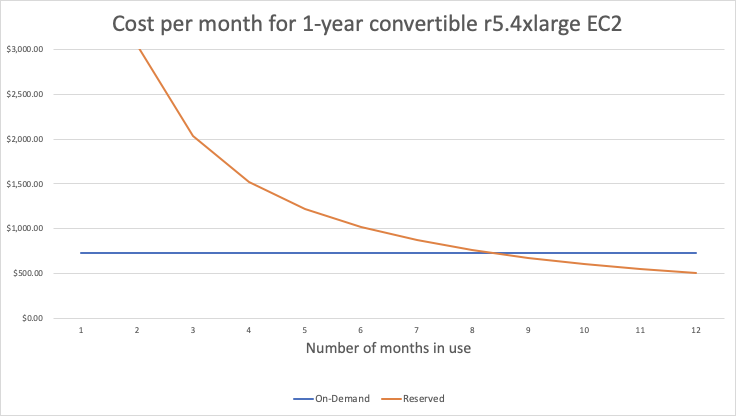
\includegraphics[scale=0.6]{sources/Kosten_RIvsOn-Demand_pro_Monat_TrueCar}\label{fig:Kosten_RIvsOn-Demand_pro_Monat_TrueCar}\\
  \caption[Monatliche Kosten für eine On-Demand-Instanz im Vergleich zu einer reservierten Instanz]{}
\begin{footnotesize}
  \label{fig:Kosten_RIvsOn-Demand_pro_Monat_TrueCar}Monatliche Kosten für eine On-Demand-Instanz\\ im Vergleich zu einer reservierten Instanz.\\
  Quelle: David Wang, 2019, How TrueCar Saves 40\% on AWS with EC2 Reserved Instances. O.s.\cite{MED1}
\end{footnotesize}
\end{figure}
%In diesem Prozess haben die Entwickler von TrueCar Mitarbeiter von den Buchhaltungs- und Finanzabteilungen involviert, um die Preisvorteile zu besprechen. 
\\\\
Nach der Buchung der reservierten Instanzen wurde deren Nutzung anhand von zwei Metriken mit Cost-Explorer überwacht. 
%Mit Cost-Explorer wurden die folgenden zwei Metriken überwacht: 
\\\\
1) Der \textbf{RI-Coverage} zeigt an, wie viel der On-Demand-Instanzen durch reservierte Instanzen abgedeckt wird. Ziel ist hierbei das \textit{RI-Coverage} (Abdeckung der reservierten Instanzen) so nahe wie möglich an 100\% zu halten.
\\\\
2) Die \textbf{RI-Utilization} zeigt an, wie viel Prozent der reservierten Instanzen verbraucht wurden. Hierbei wird versucht, die RI-Utilization nicht zu niedrig zu halten. Stattdessen sollte die Nutzung von On-Demand-Instanzen gering gehalten werden. 
\\\\
Der kürzlich vorgestellte Anwendungsfall hat gezeigt, wie die Verwendung reservierter Instanzen zu erheblichen Einsparungen bei TrueCar Inc. geführt hat. Ein wesentlicher Bestandteil dieser Optimierungsstrategie ist die Berechnung des Break-Even-Point, um zu wissen, wie viel Rechenkapazität reserviert werden sollte. Außerdem wurden die dafür nötige Metriken vorgestellt, mit denen die Ergebnisse der Optimierungsmaßnahme überwacht werden.\footnote{Um diese Metriken im Blick zu behalten und nicht jeden Tag den Cost-Explorer aufrufen zu müssen, wurde eine Benachrichtigung an \textit{Slack} eingerichtet. Slack ist eine Messaging-App für Unternehmen. (Vgl. Slack, o.J., Was ist Slack?, o.S.\cite{SLACK}.) Dies war über die Cost-Explorer API und eine Lambda-Funktion möglich.} 

\subsection*{Vergleich der Zahlungsmodelle}
%[Rev]
Die folgende Tabelle fasst die Eigenschaften der Zahlungsmodellen für die On-Demand-, reservierte, Saving-Plans- und Spot-Instanzen zusammen und listet typische Applikationen je nach Zahlungsmodell auf.
%[Abb. VOLLSTÄNDIG?AKTUELL?]
\begin{figure}[h!]
    \centering
    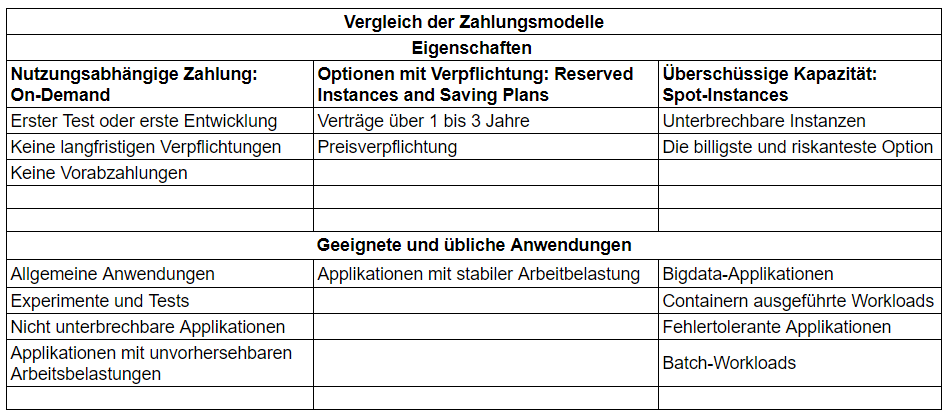
\includegraphics[scale=0.57]{sources/Vergleich_der_Zahlungsmodelle}\label{fig:Vergleich_der_Zahlungsmodelle}\\
    \caption[Vergleich der Zahlungsmodelle]{}
    \begin{footnotesize}   
    \label{fig:Vergleich_der_Zahlungsmodelle}  Vergleich der Zahlungsmodelle nach Eingenschaft und Anwendungsfall. Eigene Darstellung.\\
Quelle:Plusserver, 2021, Kostenoptimierung in AWS, S.9.\cite{PS1}\\
Spot by NetApp, 2021, What are AWS spot instances?, o.S.\cite{SPOT1}\\
AWS, 2021, On-Demand, Reserved Instances, Saving Plans and Spot-Instances, o.S.\cite{AMZ02, AMZ07, AMZ11, AMZ19}
\end{footnotesize}
\end{figure}
%
%To read planned at 21.11:
%https://www.pcapps.com/services/aws-reserved-vs-on-demand-instances/
%https://jaychapel.medium.com/aws-reserved-instances-versus-on-demand-which-is-better-e7f77f1f9582
%https://www.cloudhealthtech.com/blog/aws-reserved-instances-vs-on-demand#:~:text=In%20terms%20of%20compute%20options,of%20an%20On%20Demand%20instance.
%https://youtu.be/mKEdhmJ2udA?t=79
%Automate the selection to get the best price
%https://spot.io/aws-cost-optimization-calculator/

\newpage
\subsubsection*{Fazit}%[Rev]
In diesem Kapitel wurden die verschiedenen Zahlungsmodelle für EC2-Instanzen untersucht. Es wurden Hinweise für die Auswahl des richtigen Zahlungsmodells in verschiedenen Szenarien gegeben, um die Preisvorteile von den Zahlungsmodellen zu nutzen. Beginnend mit dem On-Demand-Zahlungsmodell, gefolgt von Reserved Instanzen und Saving Plans.\footnote{Für das On-Demand-Zahlungsmodell gibt es keine Kostenreduzierung, aber wie in Unterkapitel \ref{ssec:ZeitgesteuerteScal} gezeigt gibt Maßnahmen, um die Nutzung von Instanzen zu reduzieren.} In dieser Reihenfolge sinkt der Preis und mit ihm steigt die Verpflichtung, sich langfristig zu binden. Schließlich wurden Spot-Instanzen vorgestellt, die die niedrigsten Preise bieten, aber keine volle Verfügbarkeit sicherstellen. %In Kapitel \ref{kap_Optimierung} wird weiter auf Optimierungsmaßnahmen für EC2-Instanzen durch den Einsatz von Auto Scaling Groups eingegangen.
%[EC2-Fleet]
%En el capitulo monitoreo de costes  se mostrarán herramientas como X(CloudWatch) con las que podremos verificar si la desicion realizada fue la correcta. Para el modelo de pago On-Demand no hay ninguna redccion de los costos, pero existen medidas para aun asi reducir el uso de las instancias. Dichas medidas seran profundizadas en capitulo medidas de optimizacion
Darüber hinaus wurde ein Anwendungsfall vorgestellt, der erhebliche Einsparungen bei der Verwendung reservierter Instanzen zeigt.
\\\\
Im nächsten Kapitel werden CloudWatch, Cost-Explorer und Trusted Advisor vorgestellt. Diese Werkzeuge sollen ein besseres Verständnis über die Nutzung und Kosten von AWS-Diensten, die Analyse von Metriken ermöglichen und Empfehlungen zur Kostenoptimierung geben.
%Auf weitere Optimierungsmaßnahmen für EC2-Instanzen wird im Kapitel \ref{kap_Optimierung} näher eingegangen.